Grafičko sučelje predstavlja prikladan način za korisnika kako bi jednostavno obavljao zadatke upravljanja karticama
i pregleda dnevnika pristupa.
Prethodno definirane funkcionalnosti u pozadinskoj aplikaciji koje treba implementirati u grafičkom sučelju su:

\begin{itemize}
    \item Autorizacija korisnika
    \item Upravljanje karticama
    \item Pregled dnevnika pristupa
\end{itemize}

Aplikacije na web platformi koje se izvršavaju u pregledniku nemaju mogućnost odabira jezika.
Tri su jezika potrebna za izradu grafičkog sučelja na web platformi: HTML, CSS i JavaScript.
Pri razvoju sučelja koristi se radni okvir \textit{Vue}, a osnovne vizualne komponente pruža \textit{Vuetify}.

\subsection{Autorizacija korisnika}

Prije poduzimanja bilo kojih akcija, korisnik se mora autorizirati (prijaviti) u aplikaciju.
Forma za unos pristupnih podataka prikazana je u nastavku.

\begin{figure}[h!]
    \centering
    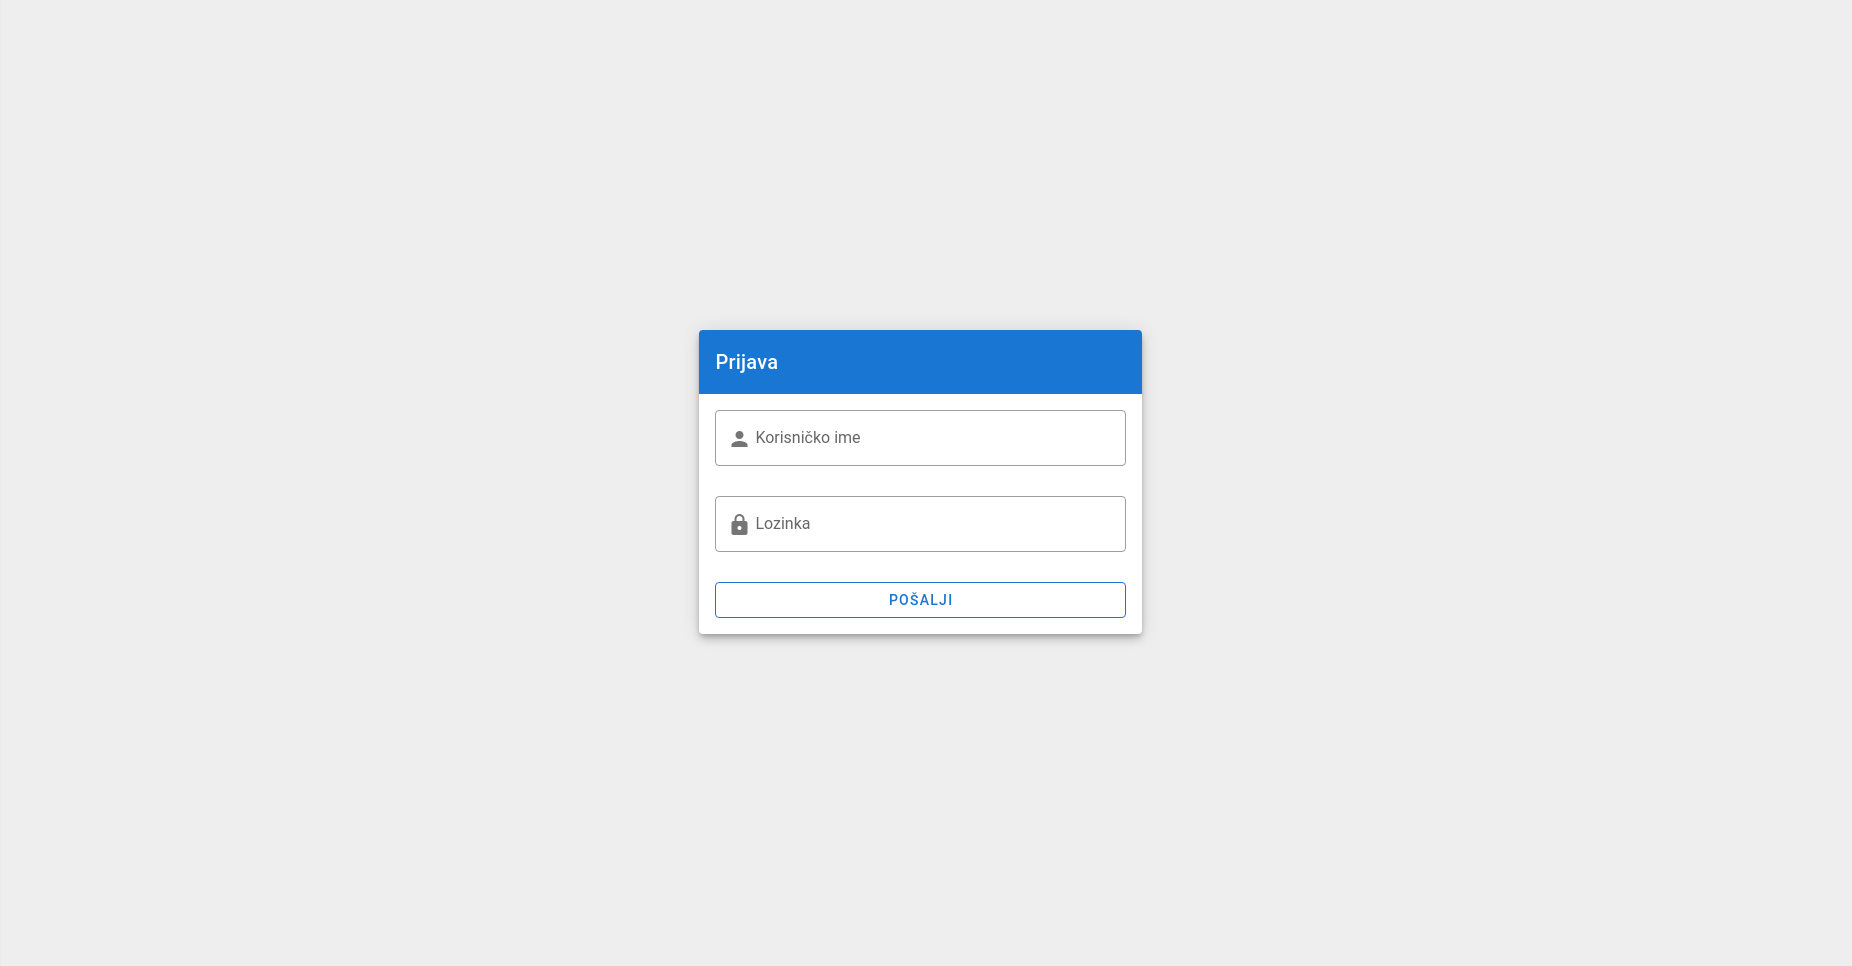
\includegraphics[width=\textwidth]{images/login-view}
    \caption{Forma za unos pristupnih podataka}
    \label{fig:login-view}
\end{figure}

\pagebreak

Na slici~\ref{fig:login-view} su tri važne komponente za obavljanje autorizacije:

\begin{enumerate}
    \item Polje za unos korisničkog imena
        \begin{lstlisting}[language=HTML]
<v-text-field
    v-model="username.value"
    label="Korisnicko ime"
    prepend-inner-icon="mdi-account"
    outlined
/>
        \end{lstlisting}
    \item Polje za unos lozinke
        \begin{lstlisting}[language=HTML]
<v-text-field
    v-model="password.value"
    type="password"
    label="Lozinka"
    prepend-inner-icon="mdi-lock"
    outlined
/>
        \end{lstlisting}
    \item Gumb za slanje zahtjeva
        \begin{lstlisting}[language=HTML]
<v-btn
    color="primary"
    type="submit"
    block
    outlined
>
    Posalji
</v-btn>
        \end{lstlisting}
\end{enumerate}

Komponente su omotane oko \textit{v-form} komponente koja je zaslužna za slanje zahtjeva kad korisnik pritisne gumb.

\begin{lstlisting}[language=HTML]
<v-form @submit.prevent="login">
</v-form>
\end{lstlisting}

Kako HTML ne može slati zahtjeve prema serveru i izvoditi bilo kakvu logiku, funkcija \textit{login} koja se okida na
\textit{submit} događaj je implementirana pomoću JavaScript jezika.

\begin{lstlisting}
import axios from 'axios'

export default {
  name: 'LoginForm',

  data: () => ({
    username: {
      value: ''
    },
    password: {
      value: ''
    }
  }),

  methods: {
    async login () {
      const { data } = await axios.post('/api/login', { username: this.username.value, password: this.password.value })
      const serverResponse = data.data

      this.loginSuccessful(serverResponse)
    },

    loginSuccessful (messageForUser) {
      this.$emit('success', messageForUser)
    }
  }
}
\end{lstlisting}

Svaka komponenta ima naziv \textbf{name}, može sadržavati podatke \textbf{data}, implementirati metode \textbf{methods} i sl.
U funkciji \textit{data} se nalazi objekt s vrijednostima polja koja korisnik mora ispuniti.
U \textit{methods} objektu je jedna metoda \textbf{login} koja je zadužena za slanje zahtjeva na pozadinsku aplikaciju.
Koristi se biblioteka \textbf{axios} jer olakšava slanje zahtjeva naspram standardnih \textit{fetch} i \textit{XMLHttpRequest} funkcija.
Nakon uspješne autorizacije metoda \textit{\$emit} emitira događaj i obavještava nadređenu komponentu.
Tada nadređena komponenta zna da može učitati pristupni dnevnik i kartice.

\begin{figure}[h!]
    \centering
    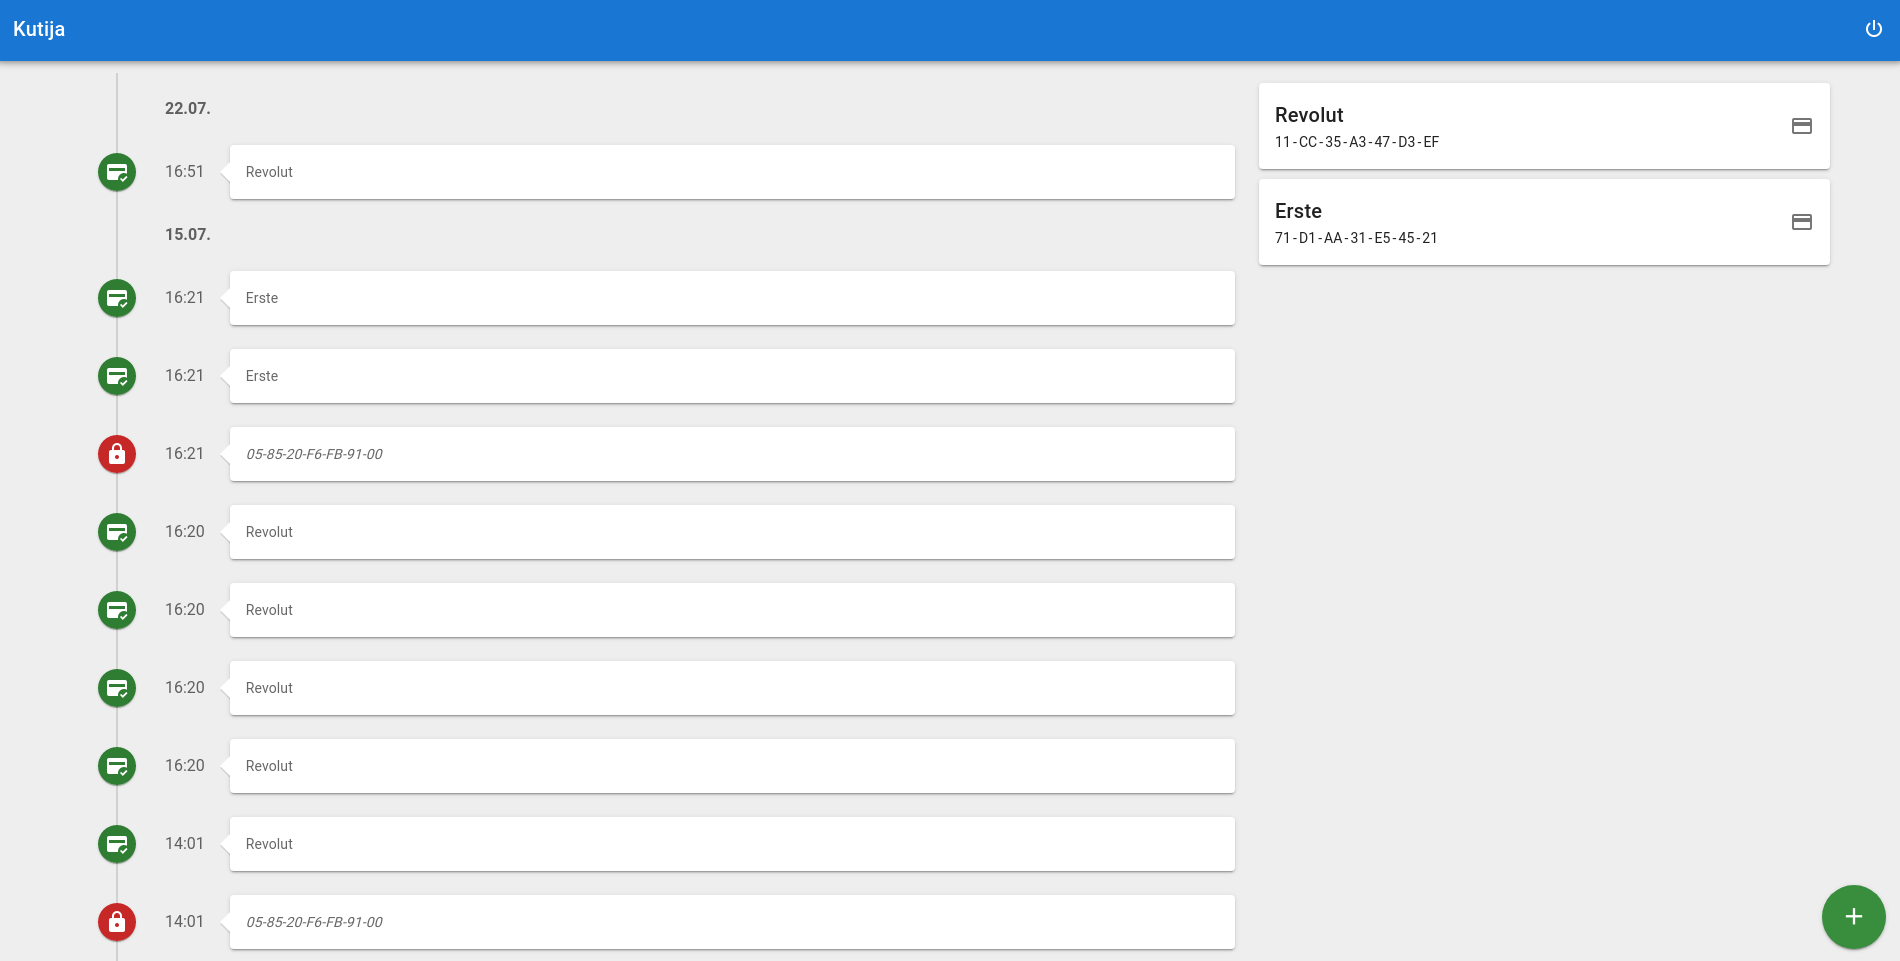
\includegraphics[width=\textwidth]{images/primary-view}
    \caption{Pristupni dnevnik i kartice}
\end{figure}
